% <<fig>> *********************************************************
\begin{figure*}[tbp]
  \unitlength1mm
  \begin{picture}(40,40)
    \centerline{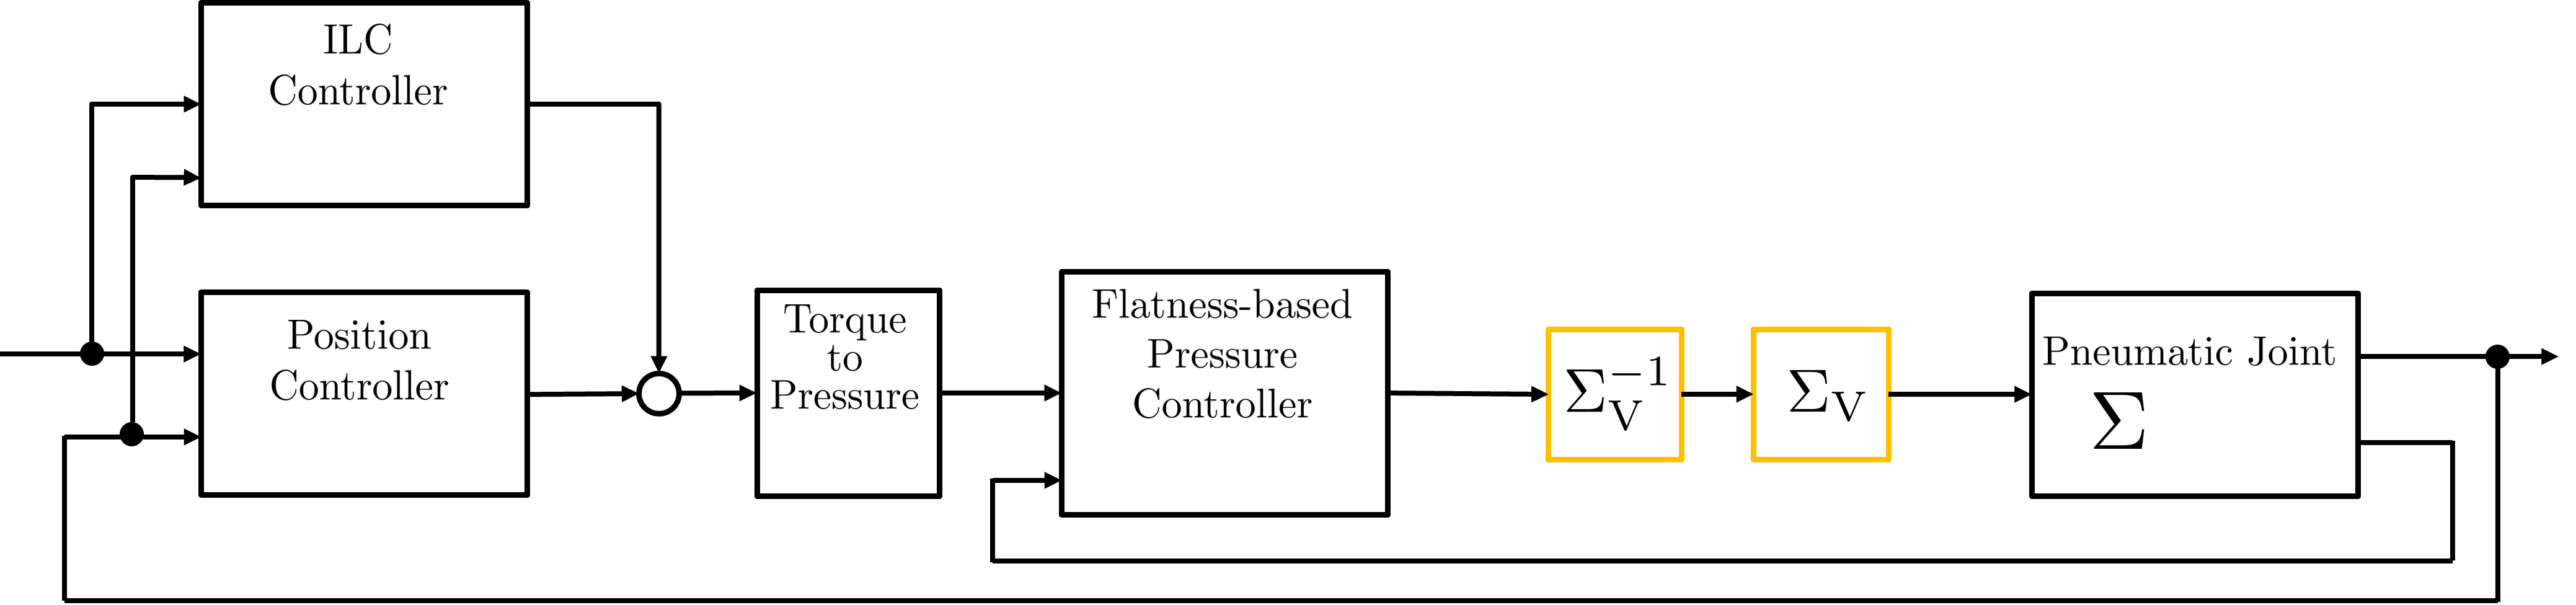
\includegraphics[scale=0.55]{./pictures/BlockSchaltFrame.png}}
    % Beschriftung von rechts nach links
    % Joint Modell *************************
    \put(-15,19){$\vp$} % Outputs
    \put(-65,4.5){$p_1,p_2$}  % KOmmt mehr in die Mitte    
    \put(-29,11.5){\eqref{pJointMdl}} % Innen
    \put(-47,16.2){$\dot m_1$} %  Inputs
    \put(-47,11){$\dot m_2$}
    % FlatnessBased Controller
    \put(-82,16.2){$\ind{\dot m}{1}$} %  Outputs
    \put(-82,11){$\ind{\dot m}{2}$}
    \put(-100,8.5){\eqref{linFB}, \eqref{linPresCtrl}} % Innen
    \put(-113,20){$\ind{p}{1,d}$} % Inputs
    \put(-113,16.5){$\ind{p}{2,d}$} % Inputs
    % Torque 2 Pressure
    \put(-124,9){\eqref{tau2pd}} 
    \put(-130.5,16){$\tau$}    % Input tau
    % Summation
    \put(-141,16){$\ind{\tau}{PI}$}    % Input tauPI
    \put(-141,36){$\ind{\tau}{ILC}$}    % Input tauILC
    % PI Pos Ctrl
    \put(-157,9.5){\eqref{taupi}}   % Eqn
    \put(-178,8){$\vp$}   % phi
    \put(-178,19){$\vpd$}   % phi
    % ILC Controller
    \put(-157,30){\eqref{eq:ilc_diskret}} % Innen    
  \end{picture}
  \caption{Overall control structure. The compensation of the valve behavior,
    \ie. $\ind{\Sigma}{V} \circ \ind{\Sigma}{V}^{-1}$, is not
    considered here.}
\label{fig:CtrlStrct}
\end{figure*}
% ******************************************************************

%%% Local Variables:
%%% mode: latex
%%% TeX-master: "../robotJointILC"
%%% End:    